\documentclass{beamer}
\usetheme{Madrid}
\usecolortheme{dolphin}
\usepackage{graphicx}
\usepackage{hyperref}

\usepackage{tikz}

\title{Enterprise Infrastructure Security}
\subtitle{Principles and Implementation}
\author{Brendan Shea, PhD}
\date{\today}

\begin{document}

\begin{frame}
    \titlepage
\end{frame}

\begin{frame}
    \frametitle{Enterprise Security: Principles \& Fundamentals}
    \begin{itemize}
        \item Security principles help organizations protect valuable information assets and infrastructure from threats.
        \item \textbf{Defense in depth} is a strategy that employs multiple layers of security controls throughout the infrastructure.
        \item Effective security requires balancing protection with usability to avoid hindering business operations.
        \item Security planning should be proactive rather than reactive, anticipating threats before they materialize.
    \end{itemize}
    
    \begin{alertblock}{Key Security Principles}
        Confidentiality, Integrity, Availability (CIA triad) forms the foundation of information security planning.
    \end{alertblock}
\end{frame}

\begin{frame}
    \frametitle{Infrastructure Security: The Big Picture}
    \begin{itemize}
        \item Enterprise infrastructure encompasses all hardware, software, networks, and services supporting business operations.
        \item Security must be considered across all infrastructure components, not just at network boundaries.
        \item \textbf{Asset inventory} is the process of identifying and documenting all components requiring protection.
        \item Threat modeling helps identify potential vulnerabilities specific to your infrastructure.
    \end{itemize}
    
    \begin{exampleblock}{Infrastructure Components}
        Servers, endpoints, network devices, cloud services, applications, databases, and physical facilities
    \end{exampleblock}
\end{frame}

\begin{frame}
    \frametitle{Strategic Device Placement: Creating Secure Architecture}
    \begin{itemize}
        \item Device placement directly impacts the security posture of the enterprise network.
        \item \textbf{Choke points} are strategic network locations where traffic can be monitored and controlled.
        \item Security devices should be positioned to maximize visibility while minimizing performance impact.
        \item Redundant security controls at critical points help maintain protection during device failures.
    \end{itemize}
    
    \begin{block}{Placement Considerations}
        \begin{itemize}
            \item Physical and logical access requirements
            \item Traffic flow patterns
            \item Resource constraints
            \item Regulatory compliance
        \end{itemize}
    \end{block}
\end{frame}

\begin{frame}
    \frametitle{Understanding Security Zones: Segmentation Strategies}
    \begin{itemize}
        \item \textbf{Security zones} are logical or physical boundaries that separate systems based on sensitivity and trust levels.
        \item Proper segmentation reduces the lateral movement capability of attackers if one zone is compromised.
        \item Traffic between zones should be strictly controlled, monitored, and limited to necessary communications.
        \item Zone design should consider both physical locations and logical data classifications.
    \end{itemize}
    
    \begin{table}
        \centering
        \begin{tabular}{|l|l|}
            \hline
            \textbf{Zone Type} & \textbf{Purpose} \\
            \hline
            DMZ & Internet-facing services with limited trust \\
            \hline
            Internal & Business operations, higher trust level \\
            \hline
            Restricted & Sensitive systems requiring highest protection \\
            \hline
            Management & Administrative access to infrastructure \\
            \hline
        \end{tabular}
        \caption{Common Security Zone Types}
    \end{table}
\end{frame}

\begin{frame}
    \frametitle{Attack Surface Analysis: Identifying Vulnerabilities}
    \begin{itemize}
        \item \textbf{Attack surface} refers to all points where an unauthorized user can attempt to enter or extract data from the environment.
        \item Every service, protocol, interface, and application potentially expands the attack surface.
        \item Regular attack surface analysis helps identify vulnerabilities before they can be exploited.
        \item Surface reduction strategies include disabling unnecessary services and implementing strict access controls.
    \end{itemize}
    
    \begin{alertblock}{Attack Surface Components}
        Network interfaces, services, protocols, open ports, APIs, user interfaces, authentication mechanisms, and third-party connections all contribute to the attack surface.
    \end{alertblock}
\end{frame}

\begin{frame}
    \frametitle{Connectivity Planning: Security Considerations}
    \begin{itemize}
        \item Connectivity planning must balance necessary business communications with security requirements.
        \item \textbf{Network traffic flows} should be carefully designed and documented to enable proper security controls.
        \item Connection points between different trust domains require special attention and robust controls.
        \item Both internal and external connectivity paths need security evaluation and appropriate protections.
    \end{itemize}
    
    \begin{exampleblock}{Connectivity Security Checklist}
        \begin{itemize}
            \item Encryption for sensitive data in transit
            \item Authentication for all connection requests
            \item Regular review of connectivity requirements
            \item Monitoring of unusual traffic patterns
        \end{itemize}
    \end{exampleblock}
\end{frame}

\begin{frame}
    \frametitle{Failure Modes: Fail-Open vs. Fail-Closed Systems}
    \begin{itemize}
        \item Security devices must be configured with appropriate behavior during failure scenarios.
        \item \textbf{Fail-open} systems allow traffic to pass without inspection when the security control fails, prioritizing availability over security.
        \item \textbf{Fail-closed} systems block all traffic when the security control fails, prioritizing security over availability.
        \item Failure mode selection depends on the criticality of the protected systems and business impact of downtime.
    \end{itemize}
    
    \begin{columns}
        \begin{column}{0.48\textwidth}
            \begin{block}{Fail-Open Use Cases}
                Load balancers, redundant systems, non-critical services
            \end{block}
        \end{column}
        \begin{column}{0.48\textwidth}
            \begin{block}{Fail-Closed Use Cases}
                Financial systems, confidential data stores, regulatory environments
            \end{block}
        \end{column}
    \end{columns}
\end{frame}

\begin{frame}
    \frametitle{Device Attributes: Active vs. Passive Security Controls}
    \begin{itemize}
        \item Security devices can be categorized by how they interact with network traffic and threats.
        \item \textbf{Active security controls} directly intervene in traffic flows, blocking or modifying suspicious communications.
        \item \textbf{Passive security controls} monitor and alert on suspicious activity without directly intervening.
        \item Both types are essential in a comprehensive security strategy to balance prevention and detection.
    \end{itemize}
    
    \begin{block}{Comparison of Active vs. Passive Controls}
        \begin{tabular}{|p{0.45\textwidth}|p{0.45\textwidth}|}
            \hline
            \textbf{Active Controls} & \textbf{Passive Controls} \\
            \hline
            Firewalls, IPS, WAF, NAC & IDS, SIEM, NBA, Honeypots \\
            \hline
            Can prevent attacks in real-time & Only detect and alert on suspicious activity \\
            \hline
            May impact performance or cause disruption & Minimal performance impact on production traffic \\
            \hline
        \end{tabular}
    \end{block}
\end{frame}

\begin{frame}
    \frametitle{Inline vs. Tap/Monitor Devices: Deployment Strategies}
    \begin{itemize}
        \item Security device deployment methods affect their capability, reliability, and performance impact.
        \item \textbf{Inline devices} process all traffic that passes through them before forwarding to the destination.
        \item \textbf{Tap/monitor devices} receive a copy of the traffic without being in the direct communication path.
        \item Deployment choice depends on whether prevention or detection is the primary goal.
    \end{itemize}
    
    \begin{alertblock}{Inline Deployment Considerations}
        Inline deployments introduce potential points of failure and latency but allow for active threat prevention. Always consider redundancy options and performance impacts.
    \end{alertblock}
\end{frame}

\begin{frame}
    \frametitle{Jump Servers: Secure Access to Critical Systems}
    \begin{itemize}
        \item \textbf{Jump servers} (or bastion hosts) are dedicated systems that provide a controlled means of accessing protected network segments.
        \item They serve as a security checkpoint between different security zones, particularly for administrative access.
        \item Jump servers should be hardened, closely monitored, and subject to strict access controls.
        \item All administrative actions should be logged and audited to maintain accountability.
    \end{itemize}
    
    \begin{exampleblock}{Jump Server Implementation}
        \begin{itemize}
            \item Located in a separate management network
            \item Multi-factor authentication required
            \item Session recording enabled
            \item Limited software installation permitted
        \end{itemize}
    \end{exampleblock}
\end{frame}

\begin{frame}
    \frametitle{Proxy Servers: Intermediaries for Enhanced Security}
    \begin{itemize}
        \item \textbf{Proxy servers} act as intermediaries between clients and destination servers, providing additional security controls.
        \item Forward proxies mediate outbound traffic from internal clients to external destinations.
        \item Reverse proxies protect internal servers by mediating inbound requests from external sources.
        \item Proxies provide benefits like content filtering, authentication, caching, and anonymity.
    \end{itemize}
    
    \begin{columns}
        \begin{column}{0.48\textwidth}
            \begin{block}{Forward Proxy Benefits}
                Content filtering, access control, bandwidth management, anonymity for internal users
            \end{block}
        \end{column}
        \begin{column}{0.48\textwidth}
            \begin{block}{Reverse Proxy Benefits}
                Load balancing, SSL termination, DDoS protection, application-layer security
            \end{block}
        \end{column}
    \end{columns}
\end{frame}


\begin{frame}
    \frametitle{IPS vs. IDS: Detecting and Preventing Intrusions}
    \begin{itemize}
        \item \textbf{Intrusion Detection Systems (IDS)} monitor network traffic for suspicious activities and generate alerts.
        \item \textbf{Intrusion Prevention Systems (IPS)} actively block detected threats in addition to generating alerts.
        \item Both systems use signature-based, anomaly-based, or behavior-based detection methods.
        \item Proper tuning is essential to minimize false positives while maintaining effective protection.
    \end{itemize}
    
    \begin{table}
        \centering
        \begin{tabular}{|l|l|l|}
            \hline
            \textbf{Characteristic} & \textbf{IDS} & \textbf{IPS} \\
            \hline
            Deployment & Passive (tap/span) & Inline \\
            \hline
            Response & Alert only & Alert and block \\
            \hline
            Latency impact & Minimal & Potentially significant \\
            \hline
            Failure impact & None (monitoring only) & Can disrupt traffic flow \\
            \hline
        \end{tabular}
        \caption{IDS vs. IPS Comparison}
    \end{table}
\end{frame}

\begin{frame}
    \frametitle{Load Balancers: Security Through Distribution}
    \begin{itemize}
        \item \textbf{Load balancers} distribute workloads across multiple computing resources to optimize resource use and availability.
        \item Beyond traffic distribution, modern load balancers provide important security functions.
        \item They can hide internal server details, terminate encrypted connections, and provide application-layer filtering.
        \item Load balancers also help mitigate certain DDoS attacks by absorbing and distributing traffic surges.
    \end{itemize}
    
    \begin{alertblock}{Security Functions of Load Balancers}
        TLS/SSL offloading, health monitoring, session persistence, application firewall capabilities, and traffic rate limiting all enhance security posture.
    \end{alertblock}
\end{frame}

\begin{frame}
    \frametitle{Security Sensors: Detection and Monitoring}
    \begin{itemize}
        \item \textbf{Security sensors} are specialized devices or software that collect security-relevant data from the environment.
        \item Sensors may be network-based (capturing traffic) or host-based (monitoring system activities).
        \item Strategic sensor placement is crucial for comprehensive visibility across the enterprise.
        \item Collected data must be aggregated and correlated to identify complex attack patterns.
    \end{itemize}
    
    \begin{exampleblock}{Types of Security Sensors}
        \begin{itemize}
            \item Network traffic analyzers
            \item System log collectors
            \item File integrity monitors
            \item Honeypots and honeynets
        \end{itemize}
    \end{exampleblock}
\end{frame}

\begin{frame}
    \frametitle{802.1X Authentication: Securing Network Access}
    \begin{itemize}
        \item \textbf{802.1X} is an IEEE standard that provides port-based network access control at the data link layer.
        \item It prevents unauthorized devices from accessing the network even before receiving an IP address.
        \item The standard uses a client-server model with three main components: supplicant, authenticator, and authentication server.
        \item 802.1X works across wired and wireless networks, providing consistent access control.
    \end{itemize}
    
    \begin{figure}
        \centering
        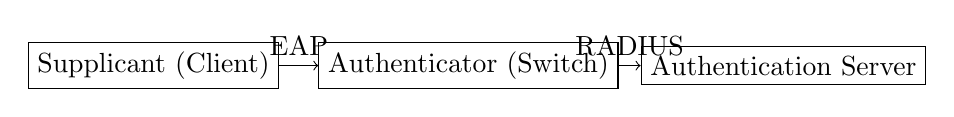
\begin{tikzpicture}[node distance=2cm]
            \node (client) [draw, rectangle] {Supplicant (Client)};
            \node (switch) [draw, rectangle, right of=client, xshift=2cm] {Authenticator (Switch)};
            \node (server) [draw, rectangle, right of=switch, xshift=2cm] {Authentication Server};
            
            \draw[->] (client) -- node[above] {EAP} (switch);
            \draw[->] (switch) -- node[above] {RADIUS} (server);
        \end{tikzpicture}
        \caption{802.1X Authentication Flow}
    \end{figure}
\end{frame}

\begin{frame}
    \frametitle{Extensible Authentication Protocol (EAP): Implementation Guide}
    \begin{itemize}
        \item \textbf{Extensible Authentication Protocol (EAP)} is an authentication framework that supports multiple authentication methods.
        \item EAP works with 802.1X to provide flexible authentication options for network access control.
        \item Different EAP types offer varying levels of security and should be selected based on requirements.
        \item Implementation requires configuration on client devices, network equipment, and authentication servers.
    \end{itemize}

    \small
    \begin{table}
        \centering
        \begin{tabular}{|l|l|l|}
            \hline
            \textbf{EAP Type} & \textbf{Security Level} & \textbf{Key Features} \\
            \hline
            EAP-MD5 & Low & Simple password authentication, no mutual auth \\
            \hline
            EAP-TLS & Very High & Certificate-based, mutual authentication \\
            \hline
            EAP-TTLS & High & Server certificate, tunneled client auth \\
            \hline
            PEAP & High & Similar to TTLS, widely supported \\
            \hline
        \end{tabular}
        \caption{Common EAP Types}
    \end{table}
\end{frame}

\begin{frame}
    \frametitle{Firewall Fundamentals: Types and Applications}
    \begin{itemize}
        \item \textbf{Firewalls} are security systems that monitor and control network traffic based on predetermined rules.
        \item They serve as a barrier between trusted internal networks and untrusted external networks.
        \item Firewalls can be implemented as hardware appliances, software applications, or cloud services.
        \item The evolution of firewalls has added capabilities beyond simple packet filtering to address complex threats.
    \end{itemize}
    
    \begin{alertblock}{Firewall Evolution}
        Firewalls have evolved from simple packet filters to sophisticated platforms that can inspect encrypted traffic, understand application behaviors, and integrate with threat intelligence.
    \end{alertblock}
\end{frame}

\begin{frame}
    \frametitle{Web Application Firewalls: Protecting Web Services}
    \begin{itemize}
        \item \textbf{Web Application Firewalls (WAF)} are specialized firewalls that protect web applications from attacks.
        \item WAFs monitor, filter, and block HTTP/HTTPS traffic to and from web applications.
        \item They defend against common web attacks like SQL injection, cross-site scripting (XSS), and CSRF.
        \item WAFs can be deployed in three modes: network-based, host-based, or cloud-based.
    \end{itemize}
    
    \begin{exampleblock}{WAF Protection Capabilities}
        \begin{itemize}
            \item Input validation and sanitization
            \item Session protection mechanisms
            \item Cookie signing and encryption
            \item Protection against OWASP Top 10 vulnerabilities
        \end{itemize}
    \end{exampleblock}
\end{frame}

\begin{frame}
    \frametitle{Unified Threat Management: Comprehensive Protection}
    \begin{itemize}
        \item \textbf{Unified Threat Management (UTM)} combines multiple security functions into a single appliance or platform.
        \item UTM solutions typically include firewall, antivirus, anti-spam, content filtering, and intrusion prevention capabilities.
        \item They simplify security administration by providing a single management interface for multiple controls.
        \item UTM is particularly suitable for smaller organizations with limited IT security resources.
    \end{itemize}
    
    \begin{block}{UTM Benefits and Limitations}
        \begin{columns}
            \begin{column}{0.48\textwidth}
                \textbf{Benefits}
                \begin{itemize}
                    \item Simplified management
                    \item Reduced hardware costs
                    \item Consolidated logging
                    \item Vendor integration
                \end{itemize}
            \end{column}
            \begin{column}{0.48\textwidth}
                \textbf{Limitations}
                \begin{itemize}
                    \item Single point of failure
                    \item Performance bottlenecks
                    \item Feature depth vs. breadth
                    \item Scalability challenges
                \end{itemize}
            \end{column}
        \end{columns}
    \end{block}
\end{frame}

\begin{frame}
    \frametitle{Next-Generation Firewalls: Advanced Filtering Capabilities}
    \begin{itemize}
        \item \textbf{Next-Generation Firewalls (NGFW)} extend traditional firewall capabilities with deep packet inspection and application awareness.
        \item NGFWs can identify and control applications regardless of port, protocol, or evasive techniques.
        \item They integrate with threat intelligence services to block known malicious sources and destinations.
        \item NGFWs often include IPS capabilities, SSL/TLS inspection, and user-based policies.
    \end{itemize}
    
    \begin{alertblock}{NGFW vs. Traditional Firewalls}
        While traditional firewalls focus on port/protocol filtering, NGFWs provide application visibility, user identity awareness, and integrated threat prevention capabilities that are essential in today's complex threat landscape.
    \end{alertblock}
\end{frame}

\begin{frame}
    \frametitle{Layer 4 vs. Layer 7 Firewalls: Technical Differences}
    \begin{itemize}
        \item Firewalls can be categorized by which OSI layers they operate at, affecting their capabilities and performance.
        \item \textbf{Layer 4 firewalls} (stateful inspection) filter traffic based on transport layer information such as TCP/UDP ports and connection states.
        \item \textbf{Layer 7 firewalls} (application firewalls) analyze application layer protocols to detect and block suspicious traffic patterns.
        \item Higher-layer inspection provides better security but requires more processing resources.
    \end{itemize}
    
    \scriptsize
    \begin{table}
        \centering
        \begin{tabular}{|l|p{0.35\textwidth}|p{0.35\textwidth}|}
            \hline
            \textbf{Feature} & \textbf{Layer 4 Firewall} & \textbf{Layer 7 Firewall} \\
            \hline
            Inspection depth & IP addresses, ports, protocol & Application commands, content \\
            \hline
            Performance impact & Lower & Higher \\
            \hline
            Bypass difficulty & Easier (port tunneling) & Harder (deep inspection) \\
            \hline
            Use case & High-throughput environments & Security-critical applications \\
            \hline
        \end{tabular}
        \caption{Layer 4 vs. Layer 7 Firewall Comparison}
    \end{table}
\end{frame}

\begin{frame}
    \frametitle{Secure Communication Basics: Protecting Data in Transit}
    \begin{itemize}
        \item \textbf{Secure communication} refers to protecting data as it moves between systems to prevent eavesdropping or tampering.
        \item Encryption transforms readable data into an encoded format that only authorized parties can decrypt.
        \item Authentication ensures that communication endpoints are who they claim to be before data exchange begins.
        \item Integrity checks verify that data hasn't been altered during transmission.
    \end{itemize}
    
    \begin{exampleblock}{Key Secure Communication Technologies}
        \begin{itemize}
            \item \textbf{VPN}: Creates encrypted tunnels across untrusted networks
            \item \textbf{TLS/SSL}: Secures web traffic and application communications
            \item \textbf{IPsec}: Network layer security for IP communications
            \item \textbf{SSH}: Secure command-line and file transfer access
        \end{itemize}
    \end{exampleblock}
\end{frame}

\begin{frame}
    \frametitle{VPN Technologies: Creating Secure Tunnels}
    \begin{itemize}
        \item \textbf{Virtual Private Networks (VPNs)} create encrypted connections over public networks to protect data in transit.
        \item VPNs enable secure remote access to internal resources for employees working outside the office.
        \item Site-to-site VPNs connect entire networks together, allowing secure communication between different locations.
        \item Different VPN protocols offer varying levels of security, performance, and compatibility.
    \end{itemize}
    
    \begin{block}{Common VPN Types}
        \begin{description}
            \item[Remote Access VPN] Connects individual users to a corporate network
            \item[Site-to-Site VPN] Connects entire networks across locations
            \item[Client-based VPN] Requires software installation on end devices
            \item[Clientless VPN] Operates through web browsers without special software
        \end{description}
    \end{block}
\end{frame}

\begin{frame}
    \frametitle{Remote Access Security: Best Practices}
    \begin{itemize}
        \item \textbf{Remote access} solutions allow users to connect to enterprise resources from outside the corporate network.
        \item Securing remote access is critical as it creates potential entry points for attackers.
        \item Multi-factor authentication should be required for all remote access connections.
        \item Access should be granted based on the principle of least privilege, limiting users to only necessary resources.
    \end{itemize}
    
    \begin{alertblock}{Remote Access Security Checklist}
        Implement strong authentication, use encrypted connections, enforce device security requirements, monitor for suspicious activities, and establish clear access policies for all remote users.
    \end{alertblock}
\end{frame}

\begin{frame}
    \frametitle{Tunneling Protocols: How They Work}
    \begin{itemize}
        \item \textbf{Tunneling protocols} encapsulate one protocol within another to provide secure passage through untrusted networks.
        \item They create logical transmission paths between network endpoints, hiding the details of internal routing.
        \item Tunneling can provide data security, protocol translation, and network address obfuscation.
        \item Different tunneling protocols are designed for specific use cases and security requirements.
    \end{itemize}

    \scriptsize
    \begin{table}
        \centering
        \begin{tabular}{|l|l|l|}
            \hline
            \textbf{Tunneling Protocol} & \textbf{Primary Use} & \textbf{Security Features} \\
            \hline
            PPTP & Legacy VPN connections & Basic encryption (weak) \\
            \hline
            L2TP/IPsec & Remote access VPN & Strong encryption, authentication \\
            \hline
            OpenVPN & Flexible VPN solution & TLS/SSL security, certificates \\
            \hline
            SSH Tunnel & Application forwarding & Strong encryption, key-based auth \\
            \hline
            GRE & Router-to-router tunneling & No built-in encryption \\
            \hline
        \end{tabular}
        \caption{Common Tunneling Protocols}
    \end{table}
\end{frame}


\begin{frame}
    \frametitle{Transport Layer Security (TLS): Implementation Guide}
    \begin{itemize}
        \item \textbf{Transport Layer Security (TLS)} is a cryptographic protocol that provides secure communications over computer networks.
        \item TLS is the successor to SSL and is used to secure web (HTTPS), email, messaging, and other application traffic.
        \item The protocol ensures confidentiality through encryption, authenticity through certificates, and integrity through message authentication codes.
        \item Proper TLS implementation requires careful configuration to avoid known vulnerabilities.
    \end{itemize}
    
    \begin{exampleblock}{TLS Best Practices}
        \begin{itemize}
            \item Use the latest TLS version (currently TLS 1.3)
            \item Disable weak cipher suites
            \item Implement proper certificate management
            \item Enable perfect forward secrecy (PFS)
        \end{itemize}
    \end{exampleblock}
\end{frame}

\begin{frame}
    \frametitle{IPSec: Securing Network Communications}
    \begin{itemize}
        \item \textbf{Internet Protocol Security (IPSec)} is a protocol suite for securing IP communications by authenticating and encrypting each IP packet.
        \item IPSec operates at the network layer, providing protection for all applications without requiring application-specific configuration.
        \item The protocol includes two main components: Authentication Header (AH) for integrity and ESP for encryption and integrity.
        \item IPSec can be implemented in transport mode (protecting payload) or tunnel mode (protecting entire packets).
    \end{itemize}
    
    \begin{block}{IPSec Security Associations}
        Security Associations (SAs) are the foundation of IPSec security, defining the parameters for secure communications:
        \begin{itemize}
            \item Encryption and authentication algorithms
            \item Keys for these algorithms
            \item Lifetime of the security association
            \item Mode of operation (transport or tunnel)
        \end{itemize}
    \end{block}
\end{frame}

\begin{frame}
    \frametitle{SD-WAN: Modern Secure Network Architecture}
    \begin{itemize}
        \item \textbf{Software-Defined Wide Area Network (SD-WAN)} is a virtual WAN architecture that allows enterprises to use any combination of transport services.
        \item SD-WAN separates network hardware from its control mechanism, using software to manage connectivity.
        \item It provides intelligent path selection across WAN links based on application requirements and real-time network conditions.
        \item Modern SD-WAN solutions incorporate integrated security features for consistent protection across distributed environments.
    \end{itemize}
    
    \begin{alertblock}{SD-WAN Security Advantages}
        SD-WAN enhances security by providing centralized policy management, encrypted communications, network segmentation, and integrated threat protection across all connection types including broadband internet and LTE.
    \end{alertblock}
\end{frame}

\begin{frame}
    \frametitle{SASE: Cloud-Delivered Security Services}
    \begin{itemize}
        \item \textbf{Secure Access Service Edge (SASE)} combines network security functions with WAN capabilities to support secure access from any location.
        \item SASE delivers security services from the cloud rather than through on-premises hardware or virtual appliances.
        \item The model shifts security from being network-perimeter focused to user/device-identity focused.
        \item SASE provides consistent security regardless of where users, applications, or data reside.
    \end{itemize}
    
    \begin{block}{SASE Components}
        \begin{itemize}
            \item \textbf{Cloud Security}: SWG, CASB, FWaaS, DLP, ZTNA
            \item \textbf{Network Optimization}: SD-WAN, WAN optimization
            \item \textbf{Identity Management}: Contextual authentication
            \item \textbf{Unified Management}: Single policy framework
        \end{itemize}
    \end{block}
\end{frame}

\begin{frame}
    \frametitle{Selecting Security Controls: Assessment Framework}
    \begin{itemize}
        \item Security control selection should follow a structured approach based on risk assessment and business requirements.
        \item \textbf{Risk assessment} involves identifying assets, threats, vulnerabilities, and potential impacts to the organization.
        \item Controls should be selected based on their effectiveness in addressing identified risks and their alignment with the security strategy.
        \item Regular evaluation of control effectiveness helps refine the security posture over time.
    \end{itemize}
    
    \begin{exampleblock}{Control Selection Process}
        \begin{enumerate}
            \item Identify and categorize assets by criticality
            \item Assess threats and vulnerabilities
            \item Determine potential impacts and likelihood
            \item Evaluate control options (technical, administrative, physical)
            \item Select and implement appropriate controls
            \item Monitor and measure effectiveness
        \end{enumerate}
    \end{exampleblock}
\end{frame}

\begin{frame}
    \frametitle{Risk-Based Security Control Selection}
    \begin{itemize}
        \item \textbf{Risk-based security} focuses on allocating resources to protect the most critical assets based on threat likelihood and potential impact.
        \item Not all assets require the same level of protection—controls should be proportional to the value and vulnerability of the asset.
        \item Risk assessment should consider both quantitative factors (costs, probabilities) and qualitative factors (reputation, compliance).
        \item The goal is to achieve the optimal balance between security investment and risk reduction.
    \end{itemize}
    
    \small
    \begin{table}
        \centering
        \begin{tabular}{|l|p{0.7\textwidth}|}
            \hline
            \textbf{Risk Level} & \textbf{Appropriate Control Strategy} \\
            \hline
            High & Implement strong preventive, detective, and corrective controls with redundancy \\
            \hline
            Medium & Balance preventive and detective controls with incident response capability \\
            \hline
            Low & Focus on baseline controls and monitoring with standard response procedures \\
            \hline
            Very Low & Accept risk with minimal controls or consider risk transfer options \\
            \hline
        \end{tabular}
        \caption{Risk-Based Control Selection Matrix}
    \end{table}
\end{frame}

\begin{frame}
    \frametitle{Defense in Depth: Layering Security Controls}
    \begin{itemize}
        \item \textbf{Defense in depth} is a security strategy that employs multiple layers of security controls throughout the infrastructure.
        \item The approach assumes that any single control may fail, so multiple overlapping protections are necessary.
        \item Layered controls should include preventive, detective, and corrective mechanisms at different levels.
        \item The strategy increases the effort required for an attacker to compromise systems and provides more opportunities for detection.
    \end{itemize}
    
    \begin{alertblock}{Layers of Defense}
        A comprehensive defense-in-depth strategy includes physical security, network security, host security, application security, and data security—each with its own set of controls working together to protect the entire environment.
    \end{alertblock}
\end{frame}

\begin{frame}
    \frametitle{Cost-Benefit Analysis of Security Controls}
    \begin{itemize}
        \item Security investments must be justified through proper evaluation of costs against expected benefits.
        \item \textbf{Cost-benefit analysis} compares the total cost of security controls against the potential losses they prevent.
        \item Costs include acquisition, implementation, operation, maintenance, and potential business impact of controls.
        \item Benefits include reduced risk, compliance fulfillment, operational improvements, and reputational protection.
    \end{itemize}
    
    \begin{block}{Security ROI Calculation}
        \begin{columns}
            \begin{column}{0.48\textwidth}
                \textbf{Control Costs:}
                \begin{itemize}
                    \item Initial purchase
                    \item Deployment costs
                    \item Training expenses
                    \item Operational overhead
                    \item Maintenance fees
                \end{itemize}
            \end{column}
            \begin{column}{0.48\textwidth}
                \textbf{Expected Benefits:}
                \begin{itemize}
                    \item Risk reduction (ALE)
                    \item Incident prevention
                    \item Compliance value
                    \item Operational efficiency
                    \item Competitive advantage
                \end{itemize}
            \end{column}
        \end{columns}
    \end{block}
\end{frame}

\begin{frame}
    \frametitle{Enterprise Security: Putting It All Together}
    \begin{itemize}
        \item Effective enterprise security requires a comprehensive approach that addresses people, processes, and technology.
        \item Security must be aligned with business objectives and supported by leadership at all levels of the organization.
        \item Regular assessment, testing, and improvement cycles help maintain an appropriate security posture as threats evolve.
        \item Documentation, training, and awareness programs are essential for ensuring consistent application of security principles.
    \end{itemize}
    
    \begin{exampleblock}{Security Program Components}
        \begin{itemize}
            \item Governance framework and policy structure
            \item Risk management processes
            \item Technical security architecture
            \item Incident response capabilities
            \item Awareness and training programs
            \item Continuous monitoring and improvement
        \end{itemize}
    \end{exampleblock}
\end{frame}

\end{document}